\documentclass{article}
\usepackage[final]{neurips_2023}
\makeatletter
\renewcommand{\@notice}{}
\makeatother
\usepackage[utf8]{inputenc}
\usepackage[T1]{fontenc}
\usepackage{hyperref}
\usepackage{url}
\usepackage{booktabs}
\usepackage{amsfonts,amsmath,amssymb}
\usepackage{nicefrac}
\usepackage{microtype}
\usepackage{xcolor}
\usepackage{graphicx}
\usepackage{subcaption}
\usepackage{multirow}
\usepackage{enumitem}
\graphicspath{{figures/}}
\setlist{nosep,leftmargin=*}
\captionsetup{font=small,skip=3pt}
\setlength{\textfloatsep}{8pt}
\setlength{\intextsep}{6pt}
\setlength{\abovecaptionskip}{3pt}

\title{Inductive Biases, Domain Alignment, and Open-Set Recognition Beyond the IID Assumption}

\author{%
  Mubeen Ahmed (25280101)\\
  Advanced Topics in Machine Learning, Fall 2026\\
  \texttt{25280101@lums.edu.pk}
}

\begin{document}
\maketitle

\begin{abstract}

This study is focused on understanding four major ways in which deployment data violate the IID assumption for the close set. These empirical findings show that (1)~Under controlled interventions on STL-10 a frozen ResNet-50 is the most texture driven framework (shape bias 58\%), ViT-B/16 is more shape driven (79\%) and CLIP the most (88-89\%), translation although leaves the predictions intact but exposes ViT's 16 pixels patch grid in feature space. The 4$\times$4 patch shuffling hurts CLIP by 15 points while ResNet loses only 7, with representation shifts far larger than prediction changes.(2)~On PACS with Sketch as target, Source-only ERM reaches 68.2\%; adversarial alignment (DANN) gains 10.9 points while MMD alignment (DAN) achieves the lowest domain separability yet suffers negative transfer ($-$3.4), and the literal protocol (shared learning rate, biased MMD estimator) is numerically unstable for both families. (3)~Without target access, pairwise source alignment (DAN-DG) lowers source separability but removes class-discriminative information (0.68 to 0.19) and loses 1.9 points.  SAM on the other hand, reduces a common sharpness proxy and gains 2.1 points, with a $\rho$ study whose Sketch ranking contradicts source-validation ranking. (4)~On CIFAR-10 with CIFAR-100 unknowns, far unknowns are rejected far better than near ones (AUROC 0.91 vs 0.81), Mahalanobis and MSP win on far and near novelty respectively. RandAugment (GCSC) improves both closed-set accuracy and rejection, and PROSER and RPL do not improve rejection at their validation-selected checkpoints. Across tasks, lower domain discrepancy never implied better recognition and higher accuracy never implied safer rejection.
Code: \url{https://github.com/<user>/pa1-beyond-iid}.
\end{abstract}




\section{Introduction}

Generally the supervised learning assumes that the test images are drawn from the training distribution belong to a known class. A model achieve the high accuracy by exploiting any statistical cues, irrespective of whether or not that cue survives a change of texture, style, position or label space.This report focuses on the four experiments: which cues
pretrained backbones rely on (Task~1), whether unlabeled target data can align a source classifier to a new visual domain without destroying class structure (Task~2), whether invariance or local flatness helps when the target is never seen (Task~3), and whether a classifier can abstain on unknown classes (Task~4). The unifying question is what a robust
representation should \emph{preserve}, what it should become \emph{invariant} to, and when it should \emph{reject}. 

The main research questions of this study include: (1) which of shape, texture and color drive ResNet, ViT and CLIP, how sensitive are they to translation and patch shuffling, and if the representation changes align with the prediction changes? (2) How large is the Photo/Art/Cartoon$\to$Sketch gap,and does lower domain separability imply better transfer,does class-conditional alignment preserves semantics better than marginal alignment and how alignment strength trade source against target performance? (3) Do source metrics predict Sketch, does source invariance transfer, does SAM reduce sharpness and if that ranking match Sketch, and what does target access buy? (4) Lastly, how does semantic distance affect rejection, what do MSP, MLS, Energy and Mahalanobis capture, and do RandAugment or placeholders improve rejection beyond a vanilla model?


\section{Experimental setup}
\label{sec:setup}
All experiments use seed 6304 and checkpoints use only validation data; target labels (Tasks~2--3) and CIFAR-100 images (Task~4) are accessed only for final evaluation. Results are saved as CSV/JSON.

\textbf{Task 1.} We split the 5\,000 STL-10 training images 80/20 and evaluate on a balanced 500-image subset \cite{coates2011stl10}. Frozen ImageNet ResNet-50, ViT-B/16~\cite{dosovitskiy2021vit}, and OpenCLIP ViT-B/32 \cite{radford2021clip} features feed linear heads trained with AdamW ($10^{-3}$, wd $10^{-4}$, at most 50 epochs); zero-shot CLIP uses ``a photo of a \{class\}.'' All inputs share a 224$\times$224 canvas. There are four types of interventions which include grayscale, hue $+120^\circ$, translations of 0/8/16/32 pixels in four directions, and one non-identity 4$\times$4 patch permutation. AdaIN cue conflicts~\cite{huang2017adain} use six prespecified class pairs in both directions (25 each); 284/300 pass the preregistered edge and colour-statistics checks. We report accuracy, prediction consistency, cosine feature stability, and joint clean/transformed t-SNE (perplexity 30, cosine distance).

\textbf{Tasks 2--3.} On PACS~\cite{li2017pacs}, Photo, Art Painting, and Cartoon are labeled sources and Sketch is the target; each source is split 80/20. We fine-tune an ImageNet ResNet-18 with frozen BatchNorm statistics using AdamW ($10^{-4}$, wd $10^{-4}$),domain-balanced batches, and source-validation macro-F1 early stopping (at most 30 epochs). Task~2 adds 24 unlabeled Sketch images per step and compares across four dimensions Source-only, DAN~\cite{long2015dan}, DANN~\cite{ganin2016dann},and CDAN~\cite{long2018cdan}. DAN uses unbiased three-kernel RBF MMD with median bandwidth scales $\{0.5,1,2\}$ and $\lambda=1$; DANN/CDAN use a 512--256--2 discriminator and the standard scheduled gradient
reversal, with CDAN applied to $\mathrm{vec}(f\otimes p)$. We also test $\lambda_{\rm MMD}\in\{0.1,1,10\}$. Task~3 reuses the Source-only checkpoint as ERM, compares pairwise source MMD (DAN-DG, $\lambda=1$) with SAM~\cite{foret2021sam} ($\rho=0.05$), and tests $\rho\in\{0.01,0.05,0.1\}$. Diagnostics are balanced linear domain probes and the fixed-batch sharpness proxy
$L(\theta+0.05\nabla L/\|\nabla L\|)-L(\theta)$. Furthermore, it was noted that the shared $10^{-4}$ learning rate made DANN/CDAN diverge, so their discriminators use $10^{-3}$; all other settings are unchanged. Biased MMD collapsed the features, so reported MMD runs use the unbiased U-statistic~\cite{gretton2012mmd}. The failed runs remain in Table~\ref{tab:unstable}.

\textbf{Task 4.} CIFAR-10 uses a stratified 45k/5k train validation split and the full test set for closed-set accuracy \cite{krizhevsky2009cifar}. There are 800 unknown images each from eight near classes (bus, pickup truck, motorcycle, tractor, wolf, fox, leopard, camel) and eight far classes (bottle, bowl, chair, clock, keyboard, mushroom, sunflower,wardrobe) in CIFAR-100. A CIFAR ResNet-18 is trained for 100 epochs with SGD (lr 0.1, momentum 0.9, wd
$5\times10^{-4}$, cosine schedule). We compare Vanilla, GCSC~\cite{vaze2022osr} with RandAugment(2,9), PROSER~\cite{zhou2021proser} with five dummy classes and manifold mixup, and RPL~\cite{chen2020rpl} with one reciprocal point per class. MSP, MLS, Energy, Mahalanobis, and method-specific scores use identical cached features/logits; thresholds are the 95th percentile of the CIFAR-10 validation score.

\section{Task 1: Inductive Biases and Representations}

\textbf{Clean baseline.} The three heads are within 0.2 points of each other (Table~\ref{tab:t1}), so intervention effects can be compared both absolutely and relative to each model's own baseline. The CLIP head is well separated but poorly calibrated (mean confidence 0.30) because a linear layer on unit-norm embeddings produces small logits, zero-shot CLIP is 1.2 points less accurate but confident (0.94).

\textbf{Color.} Removing color costs 1.0--2.6 points; changing it costs more for every model (2.6--4.2), confirming the hypothesis that natural colour statistics are used as evidence. ResNet-50 loses the most under hue rotation (4.2 points, consistency 0.944), ViT-B/16 the least (2.6, 0.960).

\newpage
\textbf{Shape vs texture.} The results align clearly with the ordering predicted by Geirhos et al.~\cite{geirhos2019} and by later ViT studies~\cite{raghu2021,tuli2021}. ResNet-50 is the most texture-driven (shape bias 57.7\%), ViT-B/16 follows shape in 79\% of decisive cases and CLIP in 88--89\%. Coverage, however, is only 55--67\%: one third to one half of the conflicts are classified as neither class, so the shape-bias estimates rest on 156--204 decisions and the stylised STL-10 images lie far outside every backbone's training distribution. Per-pair counts (Appendix) show that the ``other'' decisions concentrate on the animal--animal pairs (bird/cat, deer/monkey), where AdaIN textures are least distinctive.





\textbf{Translation.} Predictions are essentially invariant (consistency $\ge0.977$ at 32\,px for all models,
Fig.~\ref{fig:t1curves}); reflection padding preserves the object and all backbones were trained with random crops. The representation tells a different story: ViT's stability is lower at 8\,px (0.947) than at 16 and 32\,px (0.973, 0.941), because an 8\,px shift moves content across the 16$\times$16 patch grid whereas multiples of 16 realign it, while ResNet degrades smoothly with displacement (0.969$\to$0.933) as expected from stride and pooling.


\begin{figure}[!htbp]
\centering
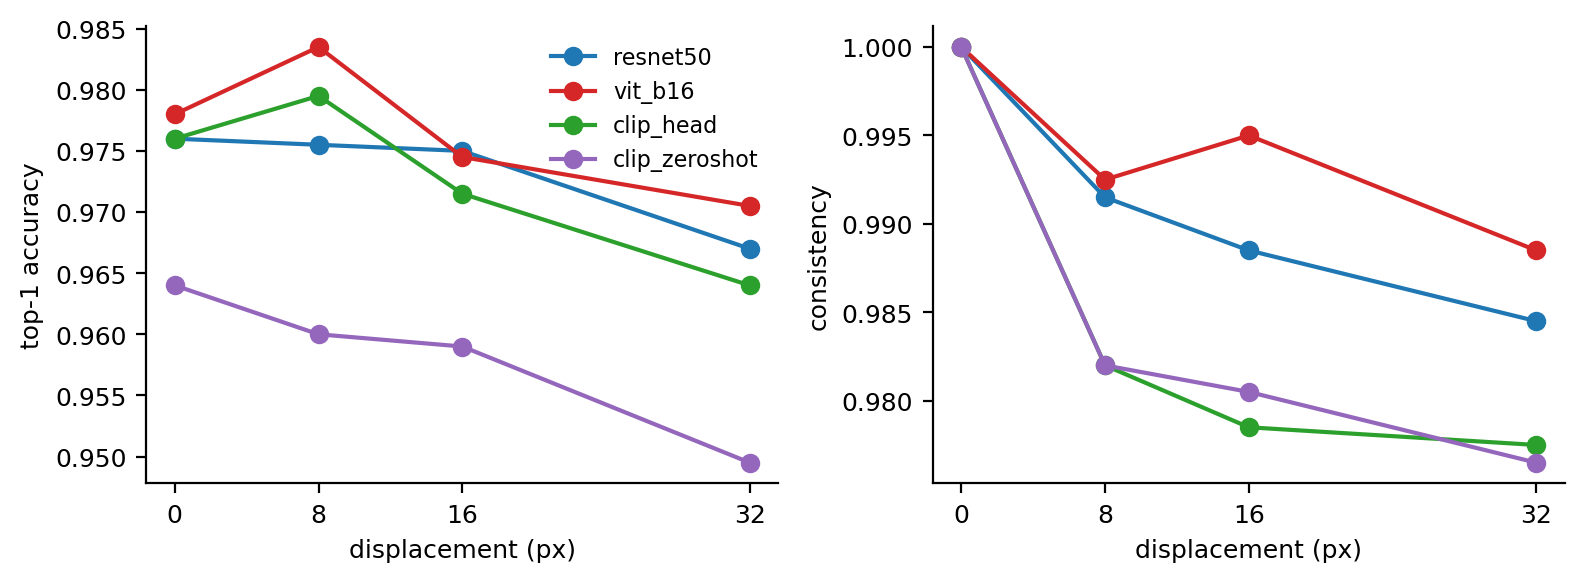
\includegraphics[width=0.49\textwidth]{task1__figures__translation_curve.png}\hfill
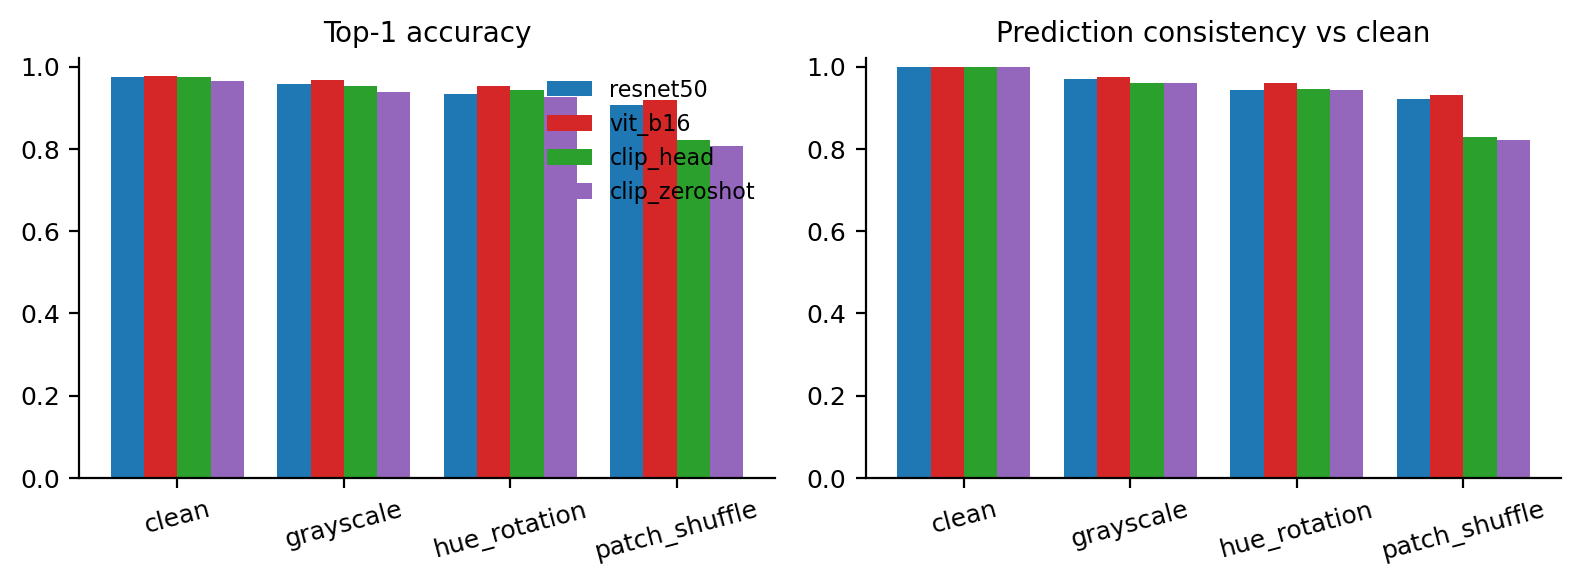
\includegraphics[width=0.49\textwidth]{task1__figures__interventions_bar.png}
\caption{Task 1. Left: accuracy and consistency versus displacement (mean over four directions). Right: accuracy and
consistency per intervention.}
\label{fig:t1curves}
\end{figure}


\textbf{Patch structure.} Shuffling the 4$\times$4 grid costs ResNet 7.0 points, ViT 6.0 and CLIP 15.4--15.8. A
56$\times$56 patch of an upscaled 96\,px image still contains large texture regions that local filters exploit, so a confident ResNet prediction after shuffling reflects surviving local evidence rather than object recognition. CLIP's embedding, trained to match captions describing whole objects, depends most on coherent layout.



\begin{table}[t]
\centering\small
\caption{Task 1. Left: top-1 (\%) / prediction consistency on the 500-image subset (clean mean max-confidence: 0.87,
0.96, 0.30, 0.94). Right: cue-conflict decisions on 284 accepted images.}
\label{tab:t1}
\setlength{\tabcolsep}{3.5pt}
\begin{tabular}{@{}lcccc@{}}
\toprule
Condition & ResNet-50 & ViT-B/16 & CLIP head & CLIP 0-shot \\
\midrule
clean & 97.6 & 97.8 & 97.6 & 96.4 \\
grayscale & 95.8/.970 & 96.8/.974 & 95.4/.960 & 93.8/.960 \\
hue $+120^\circ$ & 93.4/.944 & 95.2/.960 & 94.4/.946 & 92.6/.944 \\
patch shuffle & 90.6/.922 & 91.8/.930 & \textbf{82.2}/.830 & \textbf{80.6}/.822 \\
translate 32 & 96.7/.985 & 97.1/.989 & 96.4/.978 & 94.9/.977 \\
\bottomrule
\end{tabular}\hfill
\begin{tabular}{@{}lccccc@{}}
\toprule
Model & shape & text. & other & SB\% & Cov.\% \\
\midrule
ResNet-50 & 90 & 66 & 128 & 57.7 & 54.9 \\
ViT-B/16 & 150 & 39 & 95 & 79.4 & 66.5 \\
CLIP head & 154 & 19 & 111 & 89.0 & 60.9 \\
CLIP 0-shot & 145 & 20 & 119 & 87.9 & 58.1 \\
\bottomrule
\end{tabular}
\end{table}


\textbf{Representation analysis.} Prediction stability exceeds representation stability everywhere
(Table~\ref{tab:t1stab}). ResNet keeps 92\% of its labels under shuffling while the feature cosine drops to 0.72; grayscale and hue rotation move ViT features to 0.75/0.71 with 97\%/96\% of labels unchanged. Cue-conflict features fall to the random-pair floor for ResNet (0.258 vs 0.249) and ViT (0.230 vs 0.094 for the style image, 0.077), i.e.\ the stylised image is as far from its content source as from a random image, and slightly closer to content than to style for all three backbones. In Fig.~\ref{fig:tsne} grayscale and translated points sit on their clean clusters, cue conflicts form a mixed central blob, and for CLIP the shuffled images form \emph{separate} clusters beside the clean ones: CLIP encodes ``scrambled'' even where the label survives. Images whose label flipped had lower cosine on average (ResNet hue: 0.66 vs 0.78), so the two levels agree in tendency, but a large shift does not imply a flip. The CLIP head and zero-shot CLIP agree on every intervention because they read the same feature; the head is 1--2 points better and zero-shot is marginally more consistent.

\begin{table}[t]
\centering\small
\caption{Representation stability $I_T$ (mean cosine between clean and transformed features). ``rand.'' is the cosine
between two different clean images, the floor for each backbone.}
\label{tab:t1stab}
\setlength{\tabcolsep}{4pt}
\begin{tabular}{@{}lccccccccc@{}}
\toprule
Backbone & gray & hue & shuffle & tr.\,8 & tr.\,16 & tr.\,32 & conflict/content & conflict/style & rand. \\
\midrule
ResNet-50 & .793 & .770 & .717 & .969 & .953 & .933 & .258 & .214 & .249 \\
ViT-B/16 & .748 & .715 & .659 & \textbf{.947} & \textbf{.973} & .941 & .230 & .077 & .094 \\
CLIP ViT-B/32 & .898 & .894 & .736 & .981 & .967 & .969 & .687 & .631 & .632 \\
\bottomrule
\end{tabular}
\end{table}

\begin{figure}[t]
\centering
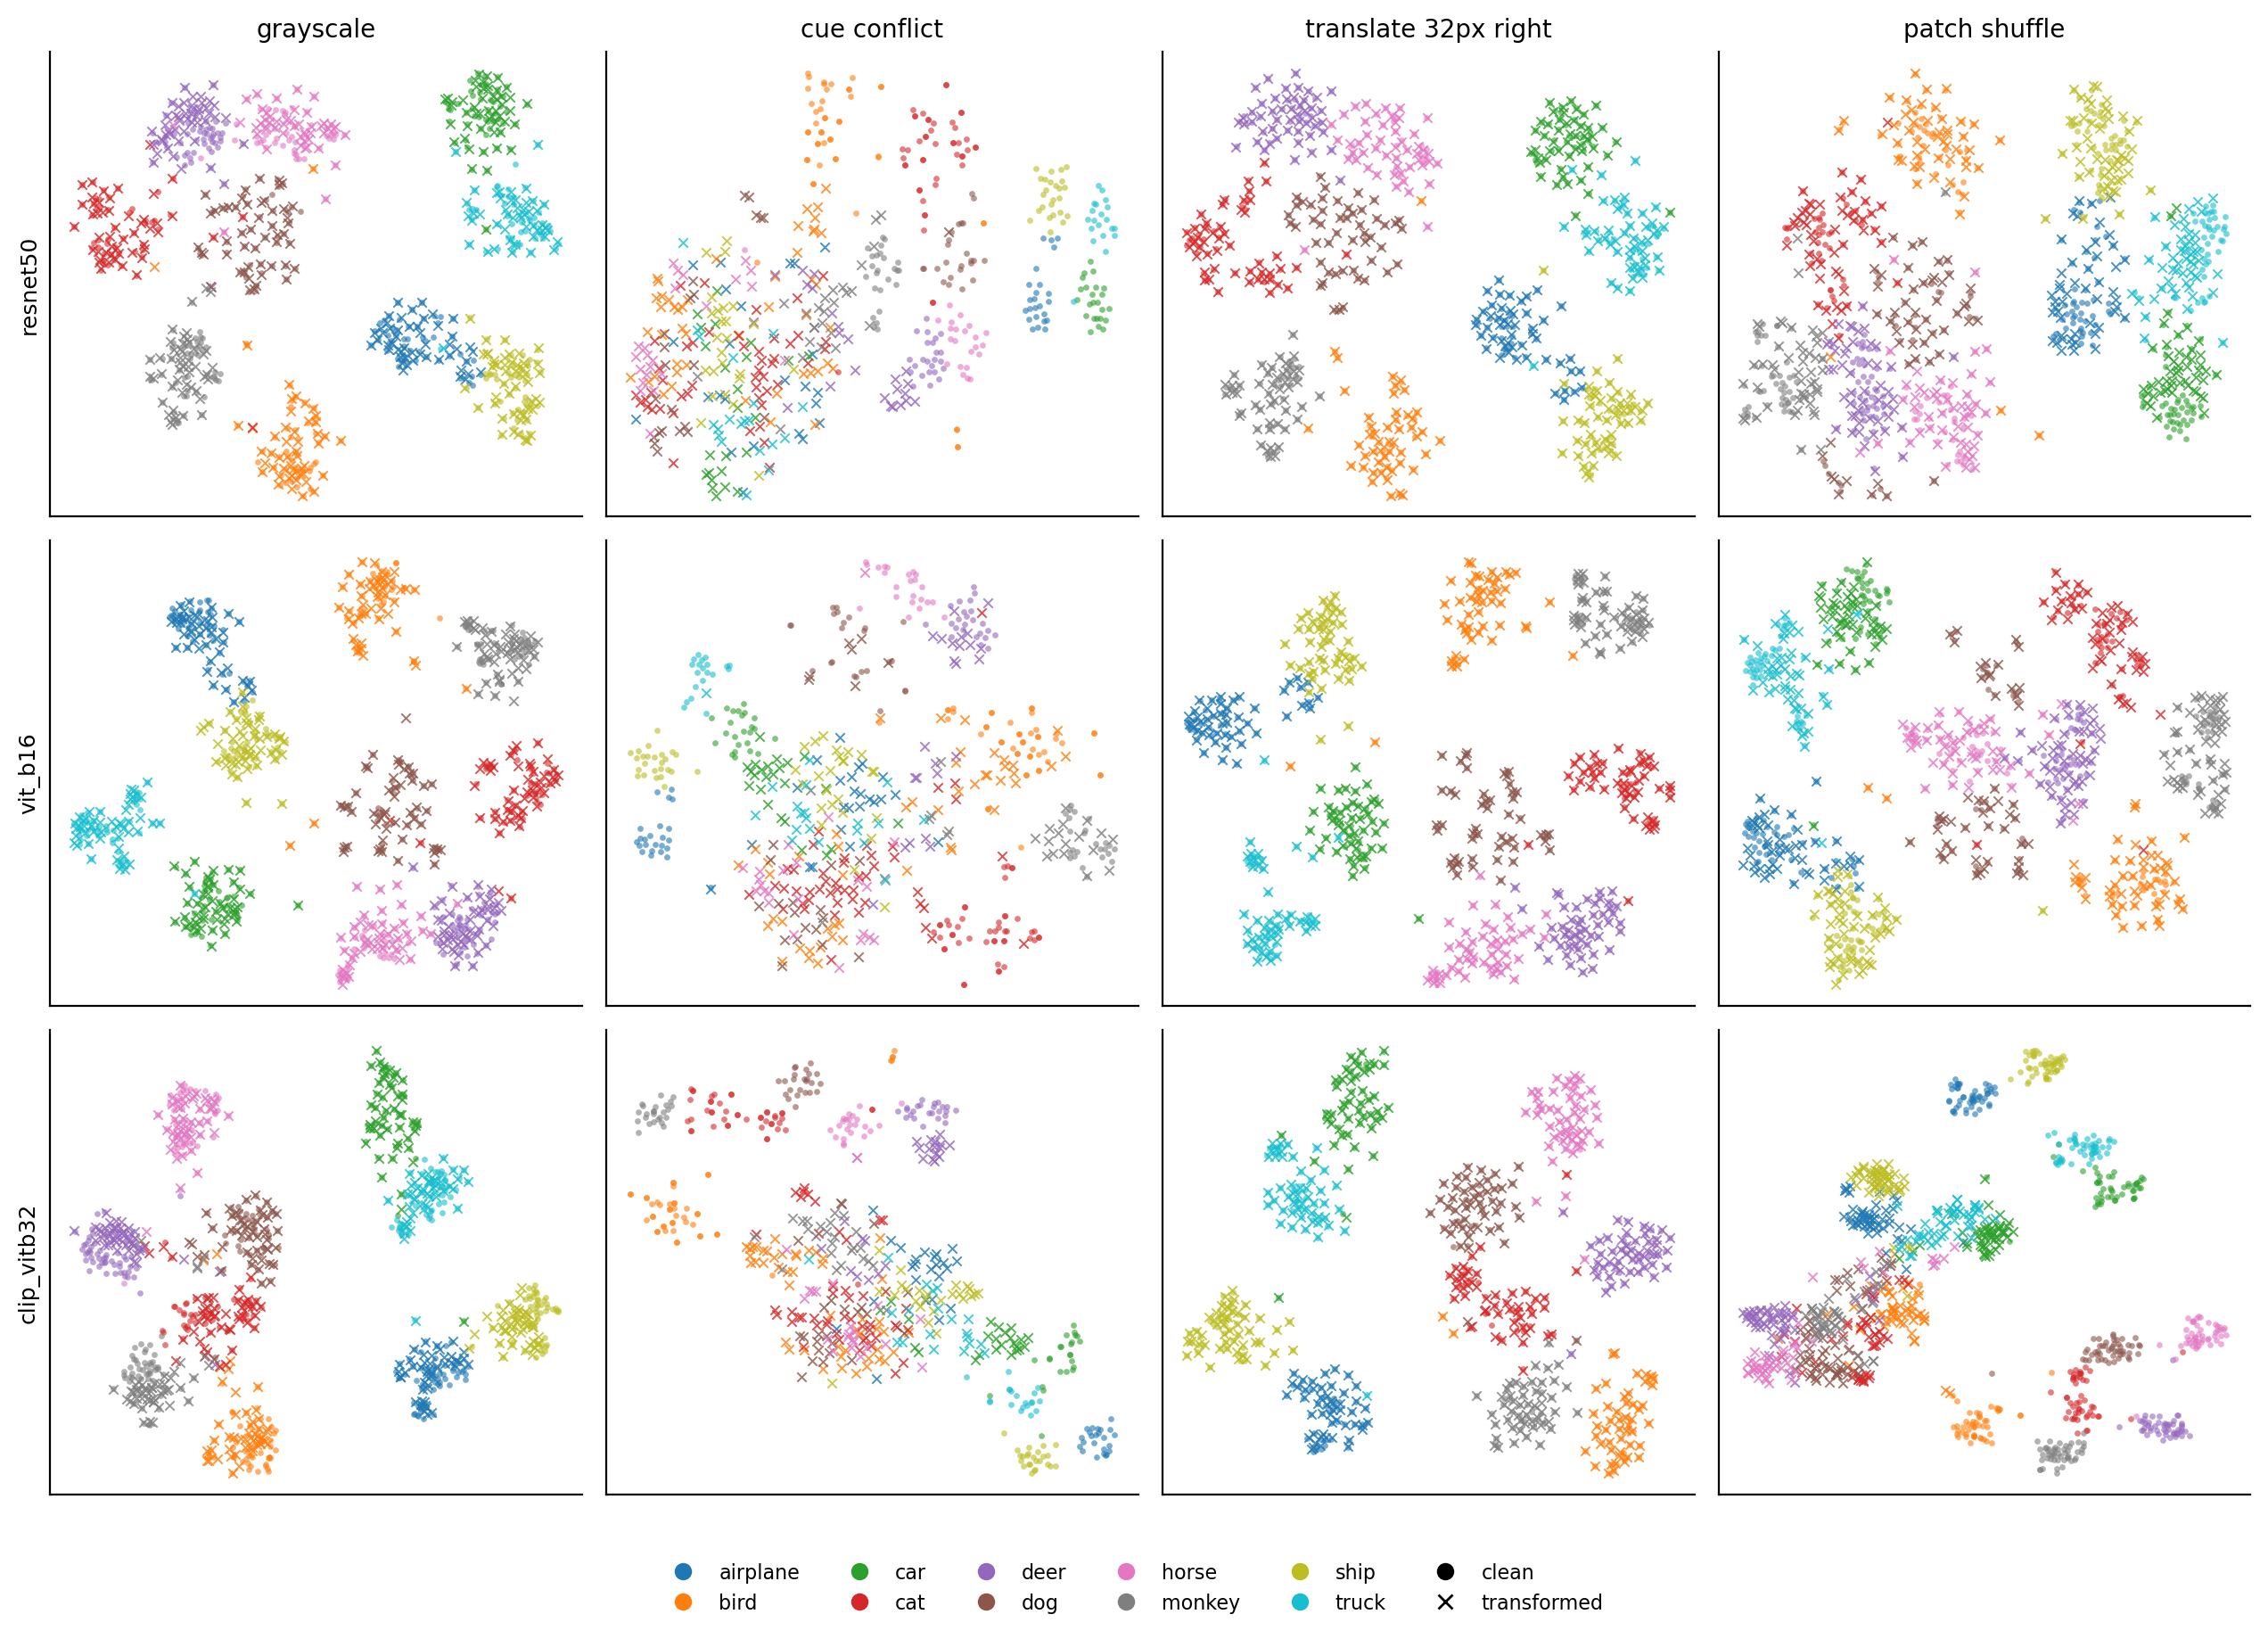
\includegraphics[width=0.99\textwidth]{task1__figures__tsne_grid.png}
\caption{t-SNE of clean ($\bullet$) and transformed ($\times$) features, one projection per panel (rows: backbones).
Colour is the ground-truth class; for cue conflicts, the shape class.}
\label{fig:tsne}
\end{figure}



Another important point is whether this results are associated to architecture or pretraining? Our results show that ResNet-50 and ViT-B/16 share ImageNet-1k supervision, so the texture bias and the smooth-versus-grid translation behavior are attributable to architecture. CLIP and ViT-B/16 share the transformer architecture, so CLIP's higher shape bias and its collapse under shuffling point to the contrastive image--text objective and its 400M-image data, with capacity, patch size (32 vs 16) and data confounded.



\section{Task 2: Unsupervised Domain Adaptation}
\begin{table}[t]
\centering\small
\caption{Task 2. Source validation macro-F1 per domain, mean source accuracy/F1, Sketch accuracy/F1, change versus
Source-only, and domain separability (50\% = chance). Bottom: controlled $\lambda_{\mathrm{MMD}}$ study.}
\label{tab:t2}
\setlength{\tabcolsep}{4pt}
\begin{tabular}{@{}lccccccccc@{}}
\toprule
Method & Photo & Art & Cartoon & Src acc & Src F1 & Sketch acc & Sketch F1 & $\Delta$acc & Sep. \\
\midrule
Source-only & .968 & .901 & .948 & .939 & .939 & .682 & .714 & -- & .997 \\
DAN ($\lambda$=1) & .966 & .905 & .949 & .940 & .940 & .649 & .607 & $-$3.4 & \textbf{.841} \\
DANN & .968 & .906 & .957 & .944 & .944 & \textbf{.791} & \textbf{.787} & \textbf{+10.9} & .988 \\
CDAN & .951 & .909 & .943 & .934 & .934 & .729 & .679 & +4.6 & .997 \\
\midrule
DAN $\lambda$=0.1 & .964 & .905 & .938 & .935 & .936 & .703 & .663 & +2.0 & .979 \\
DAN $\lambda$=10 & .954 & .884 & .893 & .913 & .910 & .706 & .659 & +2.4 & .821 \\
\bottomrule
\end{tabular}
\end{table}

\begin{table}[t]
\centering\small
\caption{Per-class Sketch accuracy (Tasks 2 and 3). Bold: largest gain / loss versus the shared ERM baseline.}
\label{tab:perclass}
\setlength{\tabcolsep}{5pt}
\begin{tabular}{@{}lccccccc@{}}
\toprule
& dog & elephant & giraffe & guitar & horse & house & person \\
\midrule
Source-only / ERM & .503 & .942 & .525 & .842 & .623 & .912 & .675 \\
DAN & \textbf{.343} & .789 & .607 & .811 & .641 & 1.00 & .912 \\
DANN & .569 & .905 & .717 & .962 & .779 & 1.00 & \textbf{.988} \\
CDAN & .528 & .880 & \textbf{.742} & .862 & .650 & 1.00 & .694 \\
\midrule
DAN-DG & .303 & .911 & \textbf{.883} & .847 & .509 & .925 & \textbf{.188} \\
SAM & .622 & .739 & .454 & .923 & .734 & .925 & .994 \\
\bottomrule
\end{tabular}
\end{table}



\textbf{Domain gap.} Source-only ERM reaches 93.9\% mean source accuracy but 68.2\% on Sketch, a 26-point gap (Table~\ref{tab:t2}). The failures (Table~\ref{tab:perclass}) are the classes whose sketches lose the texture and colour that the CNN relies on in Task~1 i.e. dog (50\%, confused with horse and person), giraffe (53\%, confused with horse) and horse (62\%); outline-defined classes (house 91\%, elephant 94\%) transfer.

\textbf{Separability versus recognition.} All four methods trained as intended (Fig.~\ref{fig:t2curves}): the MMD penalty vanishes and the domain cross-entropy converges to chance. Yet the method with by far the lowest separability. DAN (0.841), is the only one with negative transfer ($-$3.4 points; dog $-$16, elephant $-$15), while DANN leaves separability essentially unchanged (0.988) and gains 10.9 points, lifting every class and person from 0.68 to 0.99. This
is the pattern anticipated by Zhao et al.~\cite{zhao2019invariant}- matching marginal feature distributions when the label marginals differ (Sketch is dominated by dogs and people) mixes classes. And a linear probe that cannot recover the domain tells us that domain information was removed, not that class information was kept. Conversely, DANN's 512-d features still contain domain cues a supervised probe finds even though the small discriminator sat near chance during
training as the relevant alignment happened in the directions the classifier uses.

\textbf{Class-conditional versus marginal.} CDAN improves on DAN (+4.6 vs $-$3.4) and gives the largest giraffe gain (+22 points), which is consistent with conditioning aligning semantically matched regions, but it falls short of DANN and its best checkpoint arrives at epoch~3 with early stopping at~8. The 3\,584-d conditioned input makes the adversarial game harder to keep stable even with the discriminator learning-rate fix. Person value stays at 0.69 whereas DANN reaches 0.99. The evidence for ``conditioning preserves semantic structure'' is therefore partial. The CDAN avoids DAN's class mixing but does not exploit the target as well as unconditioned adversarial alignment.

\begin{figure}[!htbp]
\centering
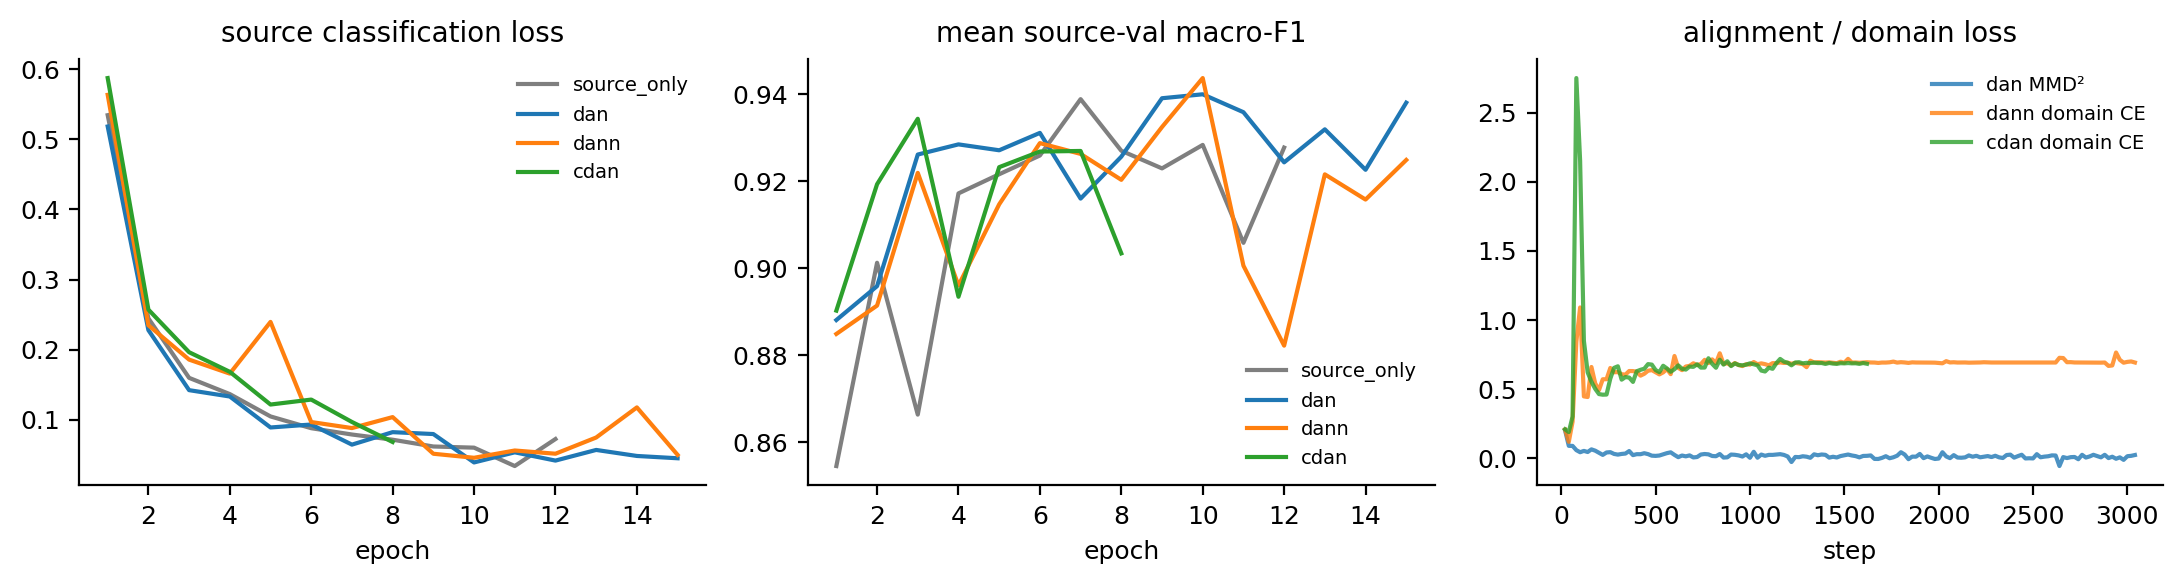
\includegraphics[width=0.99\textwidth]{task2__final_main__training_curves.png}
\caption{Task 2 training curves: source classification loss, mean source-validation macro-F1 (checkpoint criterion), and
alignment losses. DAN's MMD$^2$ reaches $\approx0$; DANN/CDAN domain cross-entropy settles at $\ln2$ after an early
spike while discriminator accuracy falls from 0.77 to 0.56--0.60 (Appendix).}
\label{fig:t2curves}
\end{figure}

\textbf{Alignment strength.} Before running the study we expected larger $\lambda$ to lower separability and source accuracy and to help the target up to a point. Separability fell monotonically (0.979, 0.841, 0.821) and source F1 dropped clearly at $\lambda=10$ (0.910), but Sketch accuracy was non-monotonic (+2.0, $-$3.4, +2.4). Selecting $\lambda$ by mean source-validation F1, the only signal permitted without target labels, would have picked $\lambda=1$ (0.940), the worst target setting. Source validation is a poor model-selection signal for UDA in this protocol.

The Table~\ref{tab:unstable} shows the instability under the literal protocol. The spec-exact adversarial runs (discriminator at $10^{-4}$) and the biased-MMD runs: source F1 collapses to 0.05--0.22 and Sketch accuracy to 4--8\%. Their separability scores (0.57--0.99) are uninformative because the features are degenerate, which illustrates the assignment's warning that chance-level discriminator accuracy can mean collapse rather than confusion.


\newpage
\section{Task 3: Domain Generalization}

The first part was to test if source metrics predict Sketch? It does only weakly (Table~\ref{tab:t3}). SAM has the best mean and worst source F1 and is also better on Sketch (+2.1), but DAN-DG slightly exceeds ERM on every source domain while losing 1.9 points on Sketch, and inside the $\rho$ study the source ranking (0.05 $>$ 0.01 $>$ 0.1) is the reverse of the Sketch ranking. Art Painting is the worst source for every model and does not discriminate between them. Class-level failures invisible in the aggregates: DAN-DG's person accuracy collapses from 0.68 to 0.19 and dog from 0.50 to 0.30 while giraffe jumps to 0.88; SAM trades elephant ($-$20) for person (+32) and horse (+11).


\begin{table}[!htbp]
\centering\small
\caption{Task 3. Source validation macro-F1 per domain, mean and worst source, Sketch accuracy/F1, change versus ERM,
3-way source-domain separability (33\% = chance) and the sharpness proxy $\Delta$. Bottom: $\rho$ study.}
\label{tab:t3}
\setlength{\tabcolsep}{3.5pt}
\begin{tabular}{@{}lcccccccccc@{}}
\toprule
Method & Photo & Art & Cartoon & Mean F1 & Worst F1 & Sketch acc & Sketch F1 & $\Delta$acc & Src sep. & $\Delta_{\rm sharp}$ \\
\midrule
ERM & .968 & .901 & .948 & .939 & .901 & .682 & .714 & -- & .870 & .181 \\
DAN-DG ($\lambda$=1) & .971 & .903 & .951 & .941 & .903 & .664 & .647 & $-$1.9 & \textbf{.758} & .120 \\
SAM ($\rho$=0.05) & .960 & \textbf{.934} & \textbf{.966} & \textbf{.954} & \textbf{.934} & .703 & .721 & +2.1 & .884 & .114 \\
\midrule
SAM $\rho$=0.01 & .972 & .892 & .974 & .946 & .892 & .714 & .722 & +3.2 & .864 & .223 \\
SAM $\rho$=0.1 & .965 & .885 & .950 & .934 & .885 & \textbf{.726} & \textbf{.739} & +4.4 & .804 & \textbf{.101} \\
\bottomrule
\end{tabular}
\end{table}


\textbf{Source Invariance Transfer} DAN-DG did what it was asked, the pairwise MMD in Fig.~\ref{fig:t3} decays to $\approx0$ and source separability falls from 0.870 to 0.758. Sketch macro-F1 nevertheless drops from 0.714 to 0.647. The person collapse is direct evidence that marginal alignment across sources removed class-discriminative information. Person is the class whose appearance varies most between photographs, paintings and cartoons, so matching the marginal feature distributions squeezes exactly the features that identify it. Invariance among observed domains is not invariance to an unseen one, and it is not class invariance.

\begin{figure}[!htbp]
\centering
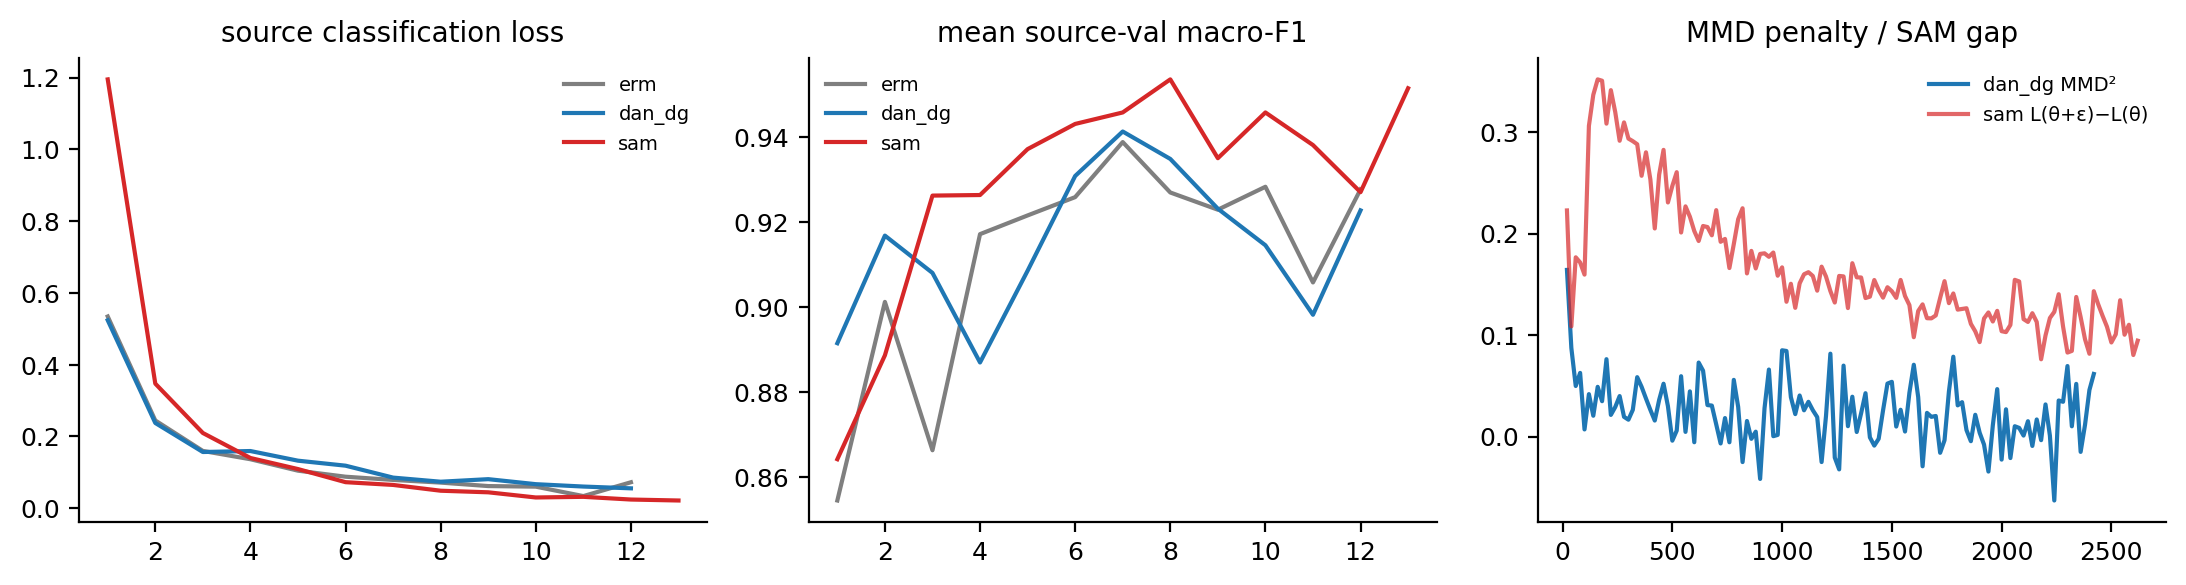
\includegraphics[width=0.62\textwidth]{task3__final_main__training_curves.png}\hfill
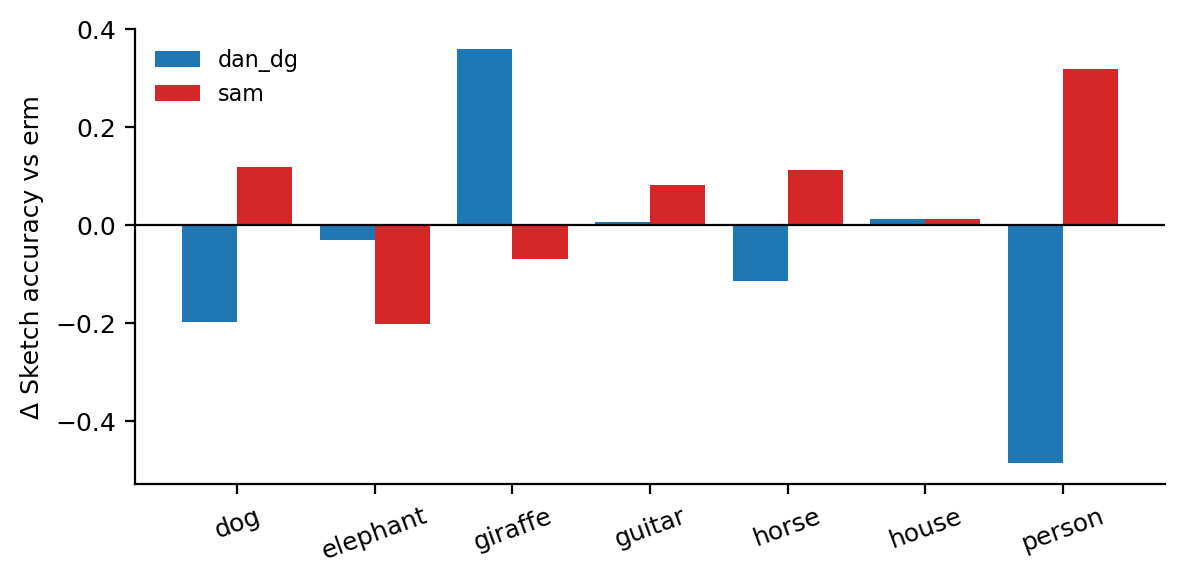
\includegraphics[width=0.37\textwidth]{task3__final_main__per_class_delta.png}
\caption{Task 3. Left: classification loss, mean source-validation F1, DAN-DG's pairwise MMD and SAM's
$L(\theta+\epsilon)-L(\theta)$ gap during training. Right: per-class Sketch change versus ERM.}
\label{fig:t3}
\end{figure}



\textbf{Sharpness.} SAM lowers the common proxy from 0.181 (ERM) to 0.114, and DAN-DG incidentally to 0.120. Across $\rho$ the proxy decreases monotonically (0.223, 0.114, 0.101) and the Sketch accuracy of the two extremes follows it (71.4 at 0.01, 72.6 at 0.1), but $\rho=0.05$ sits below both (70.3), and $\rho=0.01$ has a \emph{higher} proxy than ERM while still generalizing better. The ranking by local stability therefore agrees with the ranking by Sketch performance only at the extremes. The proxy probes one direction at one radius on 96 images and should be read as evidence about local stability, not flatness. The best Sketch setting, $\rho=0.1$, has the worst source F1 and would not have been chosen by source-only selection; the main comparison correctly retains $\rho=0.05$.

\textbf{Value of target access.} With the same ERM baseline (68.2\%) and the same unbiased MMD, target-aware DAN reached 64.9\% and target-free DAN-DG 66.4\%, both are below ERM. Unlabelled Sketch data was valuable only through the adversarial objective (DANN, +10.9), which has no target-free counterpart here. The DAN/DAN-DG pair cannot attribute the difference to access alone and the two methods align different distribution pairs (source--target versus source--source), with different samples per MMD term (24 versus 8) and different label-marginal mismatches.

\section{Task 4: Open-set Recognition}

\textbf{Semantic distance.} Every score and model rejects far unknowns much better than near ones (AUROC 0.89--0.91 vs
0.79--0.81; Table~\ref{tab:t4}, Fig.~\ref{fig:t4}). Under the Vanilla-MLS threshold ($\tau=-5.93$) the most accepted
near classes are pickup\_truck (91\%, absorbed by automobile), bus (80\%, truck 81\% of the time), wolf (80\%, cat), fox
and leopard (66--67\%, cat) and camel (61\%, deer): semantically plausible confusions. Far unknowns are also accepted at
31--59\%: wardrobe$\to$truck (73\% of accepted), chair$\to$airplane (67\%), keyboard$\to$airplane, bottle$\to$ship,
clock and bowl$\to$cat, mushroom$\to$bird. The six most confidently accepted examples per group (Appendix) have MLS
scores of $-11$ to $-13$, deep inside the known distribution; a brown box on legs is a truck and thin struts are an
aircraft to this network, echoing the coarse shape/colour reliance of Task~1.

\begin{table}[!htbp]
\centering\small
\caption{Task 4. Left: post-hoc scores on the frozen Vanilla model (CSA 94.67\%). Right: trained models with MLS, plus
PROSER's placeholder score and RPL's own score. Rejection rates are at the threshold accepting 95\% of validation
knowns; FPR@95TPR $=1-$rejection. Known test acceptance was 94.6--95.4\% in every row.}
\label{tab:t4}
\setlength{\tabcolsep}{3pt}
\begin{tabular}{@{}lccccc@{}}
\toprule
Score & AUROC near & far & all & Rej.\ near & far \\
\midrule
MSP & \textbf{.809} & .892 & .850 & .293 & .414 \\
MLS & .790 & .895 & .843 & .323 & .549 \\
Energy & .790 & .896 & .843 & .320 & .551 \\
Mahalanobis & .807 & \textbf{.910} & \textbf{.859} & .294 & .481 \\
\bottomrule
\end{tabular}\hfill
\begin{tabular}{@{}llcccccc@{}}
\toprule
Model & Score & CSA & near & far & all & Rej.\ near & far \\
\midrule
Vanilla & MLS & .947 & .790 & .895 & .843 & .323 & .549 \\
GCSC & MLS & \textbf{.951} & \textbf{.813} & \textbf{.909} & \textbf{.861} & \textbf{.354} & \textbf{.578} \\
PROSER & MLS & .944 & .793 & .880 & .837 & .293 & .460 \\
PROSER & placeh. & .944 & .774 & .861 & .817 & .283 & .451 \\
RPL & $-\max d$ & .947 & .602 & .688 & .645 & .303 & .419 \\
\bottomrule
\end{tabular}
\end{table}

\begin{figure}[!htbp]
\centering
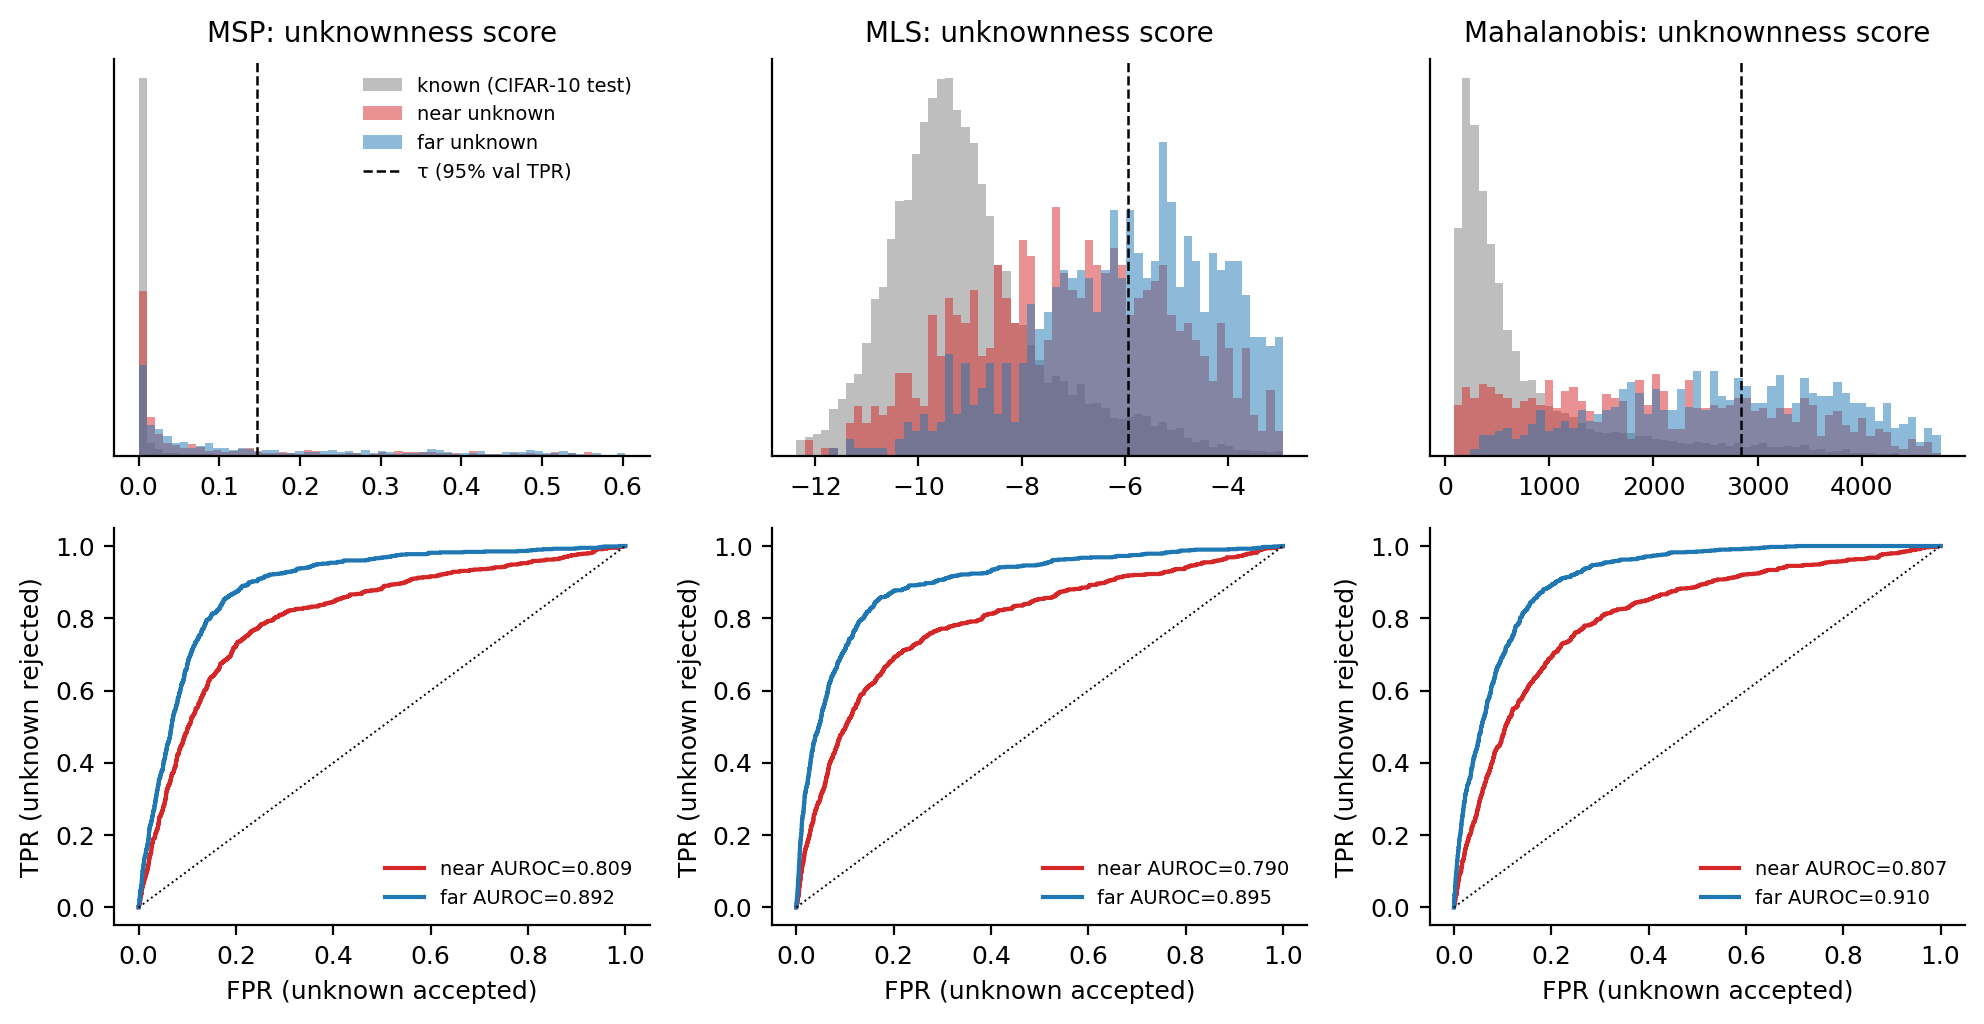
\includegraphics[width=0.99\textwidth]{task4__final__vanilla_scores_hist_roc.png}
\caption{Vanilla model: score distributions for known test, near and far unknowns (dashed: validation-calibrated
threshold) and ROC curves for MSP, MLS and Mahalanobis.}
\label{fig:t4}
\end{figure}



\textbf{What the scores capture.} MLS and Energy rank inputs almost identically (Spearman 0.9999) with one dominant logit the log-sum-exp equals the maximum. MSP correlates with them at 0.96 but is best on \emph{near} unknowns (0.809 vs 0.790) because normalization exposes competition between two known classes (bus: truck versus automobile), while MLS/Energy are better on far unknowns and reject far more of them at the operating point (55\% vs 41\%): far unknowns produce uniformly small logits that MSP cannot see after normalization. Mahalanobis, only moderately correlated with the logit scores (0.59--0.72), has the best far and overall AUROC because feature-space distance flags inputs whose logits are moderately large but whose features lie outside every class cluster. MSP's better near AUROC but lower near rejection
(29\% vs 32\%) at the calibrated threshold shows that ranking and operating-point metrics can disagree.

\textbf{GCSC.} RandAugment raised CSA by only 0.4 points but improved every open-set number, near AUROC +0.023, far +0.014, near rejection +3.1 points, far +2.9. The controlled comparison therefore supports Vaze et al.~\cite{vaze2022osr}.  A better closed-set representation makes logit magnitude a more reliable evidence measure, and the gain is slightly larger for near unknowns, where sharper boundaries between truck-like classes matter most.

\textbf{PROSER and RPL.} PROSER trained as designed (99\% of mixed features were routed to the dummy class, CSA fell steadily during fine-tuning as the placeholders tightened known regions), but the validation-accuracy rule selected epoch~8 of 50, and at that checkpoint neither MLS (0.837) nor the placeholder score (0.817) improves on Vanilla (0.843), with CSA 0.3 points lower. Two reasons are visible in the results: the Vanilla initialization already fits CIFAR-10 at
99.97\% training accuracy, leaving little gradient for the classifier-placeholder term, and interpolations between two known classes are proxy unknowns that lie on segments between CIFAR-10 clusters, whereas the far unknowns that are accepted (wardrobe, chair) do not. RPL matched Vanilla's CSA (94.7\%) but rejected poorly (AUROC 0.60/0.69) with distance-as-logit at $T=1$, any confidently classified input, known or not, is far from ``not-that-class'', so the
maximum distance carries little novelty information. Learning what each class is not did not translate into rejection
in this configuration.

\section{Cross-task discussion}
\textbf{Visual Cues and Distribution Shift.} The ImageNet CNN of Task~1 leans on texture and color statistics (lowest shape bias, largest hue-rotation loss, smallest shuffle loss). The PACS domain on which the ResNet-18 of Tasks~2--3 fails is precisely the one that removes texture and colour: source 94\% versus Sketch 68\%, with texture-defined animals failing and outline-defined classes surviving. Task~4's far-unknown failures (wardrobe$\to$truck, chair$\to$airplane) show the same coarse-shape reliance from the other direction. The comparison is qualitative, since datasets, resolutions and architectures differ.

\textbf{Invariance Versus Discriminability.} In neither Task~2 nor Task~3 did the lowest separability coincide with the best recognition. DAN (0.84) and DAN-DG (0.76) both fell below ERM and each destroyed specific classes (dog/elephant; person), whereas DANN kept separability at 0.99 and gained 11 points. Invariance removed noise where style was orthogonal to class (giraffe improved under every alignment method) and removed signal where the class is defined by
domain-specific appearance. A domain probe measures what was removed, not what was kept.

\textbf{Target-domain access.} Holding the ERM baseline and the MMD mechanism fixed, unlabeled Sketch data did not help (DAN 64.9 vs DAN-DG 66.4 vs ERM 68.2); the target-aware gain came from the adversarial objective. Access enabled a more useful kind of alignment, but the DAN/DAN-DG pair differs in the distributions aligned, the samples per estimate and the
label marginals, so it does not isolate access as the cause.

\textbf{Recognition versus rejection.} Better closed-set accuracy went with better rejection for GCSC, but PROSER lowered CSA slightly without improving rejection and RPL matched CSA while rejecting poorly; near unknowns stay hard for every method (AUROC $\le0.81$). A confident ``truck'' on a bus is where a classifier should abstain and does not.

\textbf{Synthesis.} 
\section{Conclusion}
Controlled interventions showed that the backbones relied on cues largely as predicted by prior work, while PACS revealed that representations can shift far more than predictions. The method that made domains least distinguishable transferred worst, and source-only model selection would have chosen the wrong alignment strength and SAM radius. On CIFAR, near and far novelty required different rejection scores: MSP suited ambiguous class evidence, whereas Mahalanobis distance better detected samples lying outside known feature clusters. A stronger classifier also improved rejection, while placeholder learning did not at its validation-selected checkpoint. Overall, robust representations should preserve global shape cues that survive sketches, cue conflicts, and changes in color, texture, and rendering style. However, invariance is desirable only when such factors are not class-defining, motivating class-aware rather than marginal alignment and rejection of inputs outside the known label space. Limitations include single seeds, one backbone per protocol, and diagnostics such as linear probes and a one-direction sharpness proxy, which provide evidence rather than proof.

\bibliographystyle{plainnat}
\bibliography{references}

\appendix
\section{Appendix: additional evidence}
\begin{table}[h]
\centering\small
\caption{Spec-exact and biased-estimator runs kept as evidence of optimization failure (Task 2 protocol).}
\label{tab:unstable}
\setlength{\tabcolsep}{4pt}
\begin{tabular}{@{}lcccccccc@{}}
\toprule
Run & Photo F1 & Art F1 & Cartoon F1 & Src F1 & Sketch acc & Sketch F1 & $\Delta$acc & Sep. \\
\midrule
DANN, discriminator lr $10^{-4}$ & .158 & .100 & .087 & .115 & .073 & .045 & $-$60.9 & .920 \\
CDAN, discriminator lr $10^{-4}$ & .247 & .188 & .230 & .222 & .080 & .074 & $-$60.3 & .999 \\
DAN $\lambda$=1, biased MMD & .967 & .929 & .945 & .947 & .548 & .535 & $-$13.5 & .819 \\
DAN $\lambda$=10, biased MMD & .059 & .051 & .042 & .051 & .041 & .011 & $-$64.2 & .574 \\
DAN-DG $\lambda$=1, biased MMD (Task 3) & .059 & .051 & .042 & .051 & -- & -- & -- & .395 (3-way) \\
\bottomrule
\end{tabular}
\end{table}

\begin{figure}[h]
\centering
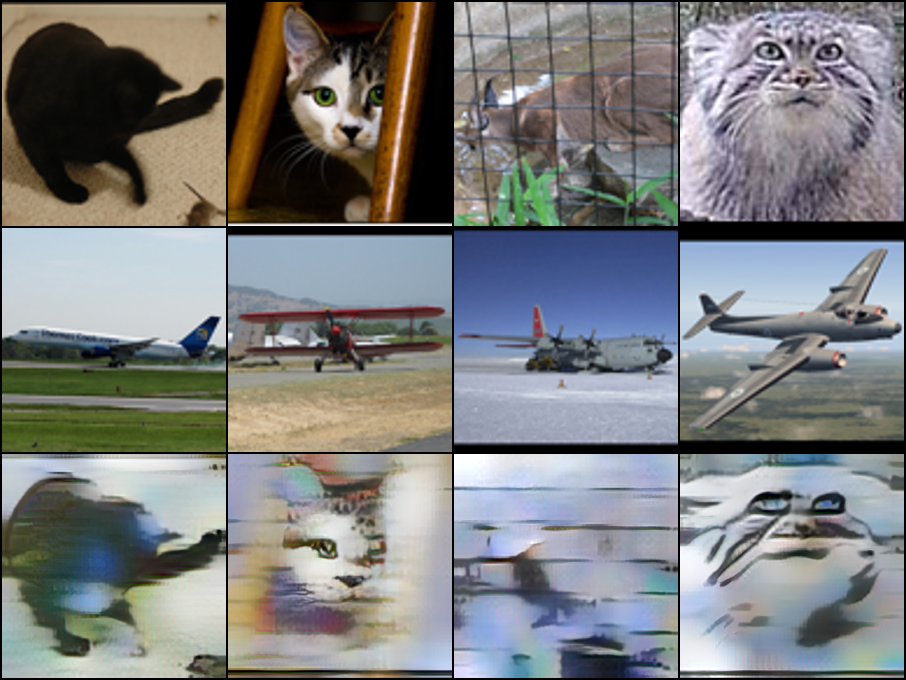
\includegraphics[width=0.48\textwidth]{task1__images__examples__triplet_cat_content__airplane_style.png}\hfill
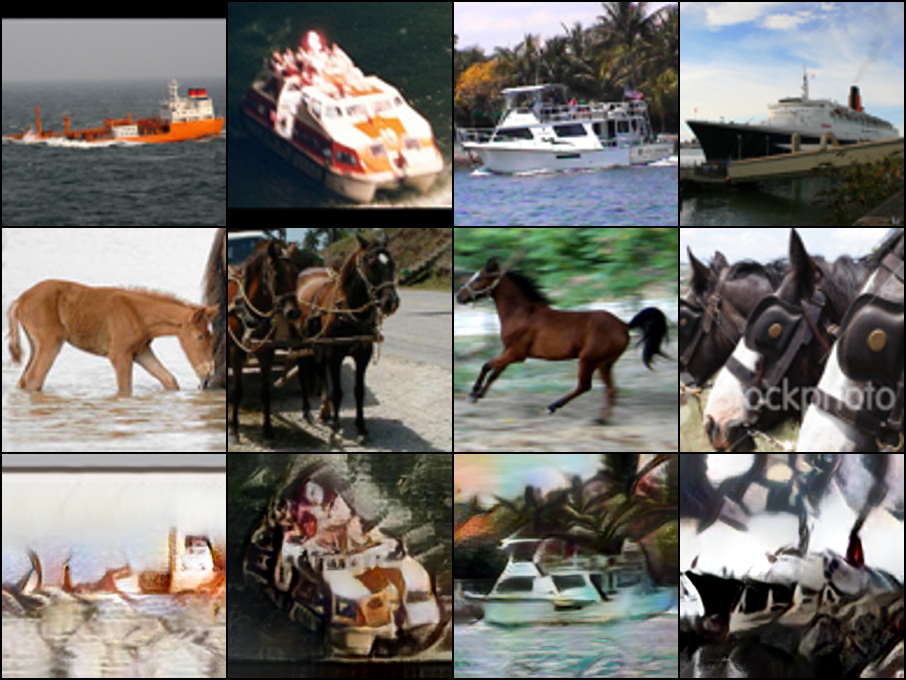
\includegraphics[width=0.48\textwidth]{task1__images__examples__triplet_ship_content__horse_style.png}
\caption{Cue-conflict examples (rows: content/shape, style/texture, AdaIN output) for cat$\times$airplane and
ship$\times$horse.}
\end{figure}

\begin{figure}[h]
\centering
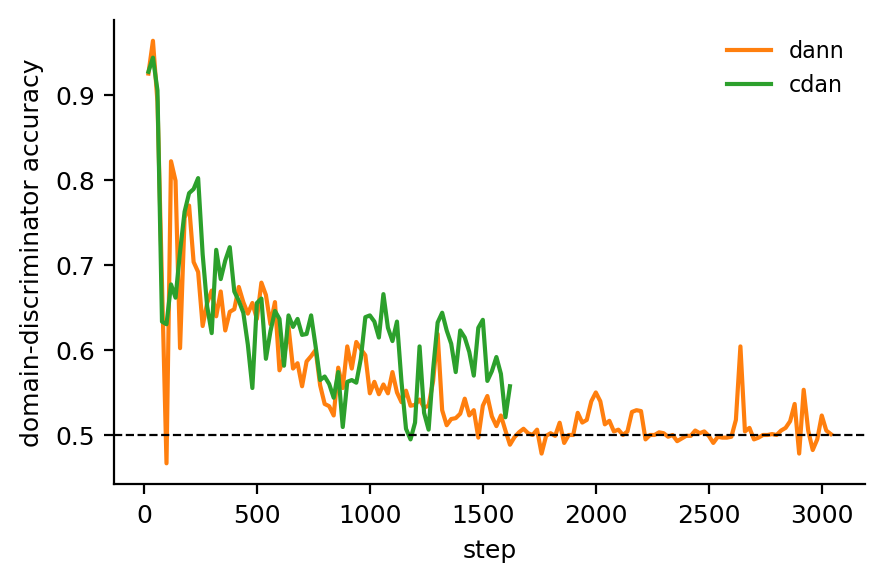
\includegraphics[width=0.32\textwidth]{task2__final_main__discriminator_acc.png}\hfill
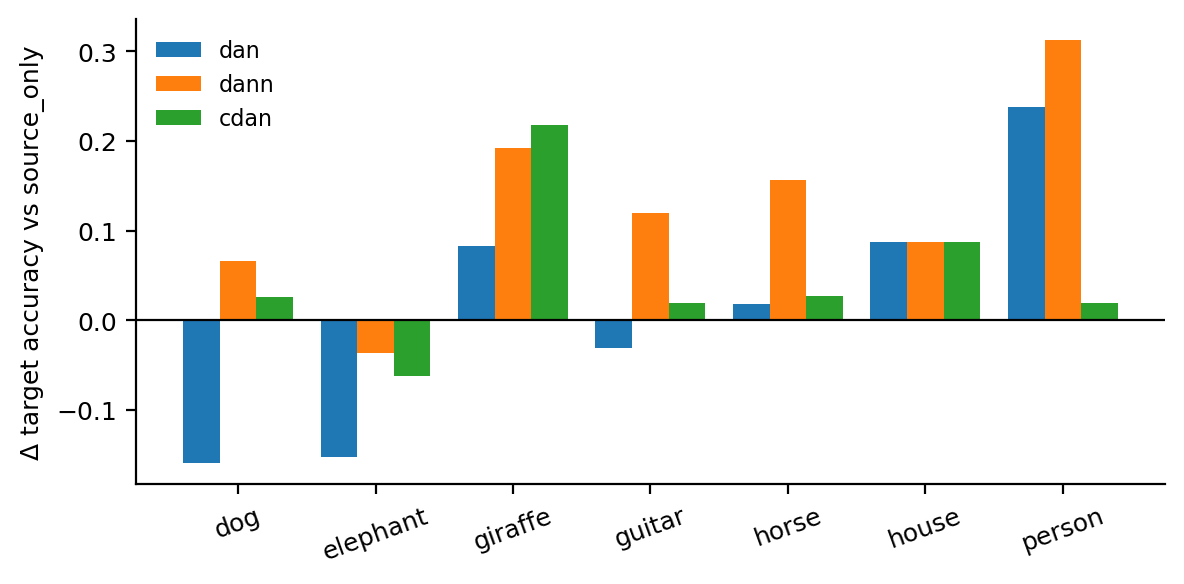
\includegraphics[width=0.66\textwidth]{task2__final_main__per_class_delta.png}
\caption{Task 2: domain-discriminator accuracy during training (left) and per-class Sketch change versus Source-only (right).}
\end{figure}

\begin{figure}[h]
\centering
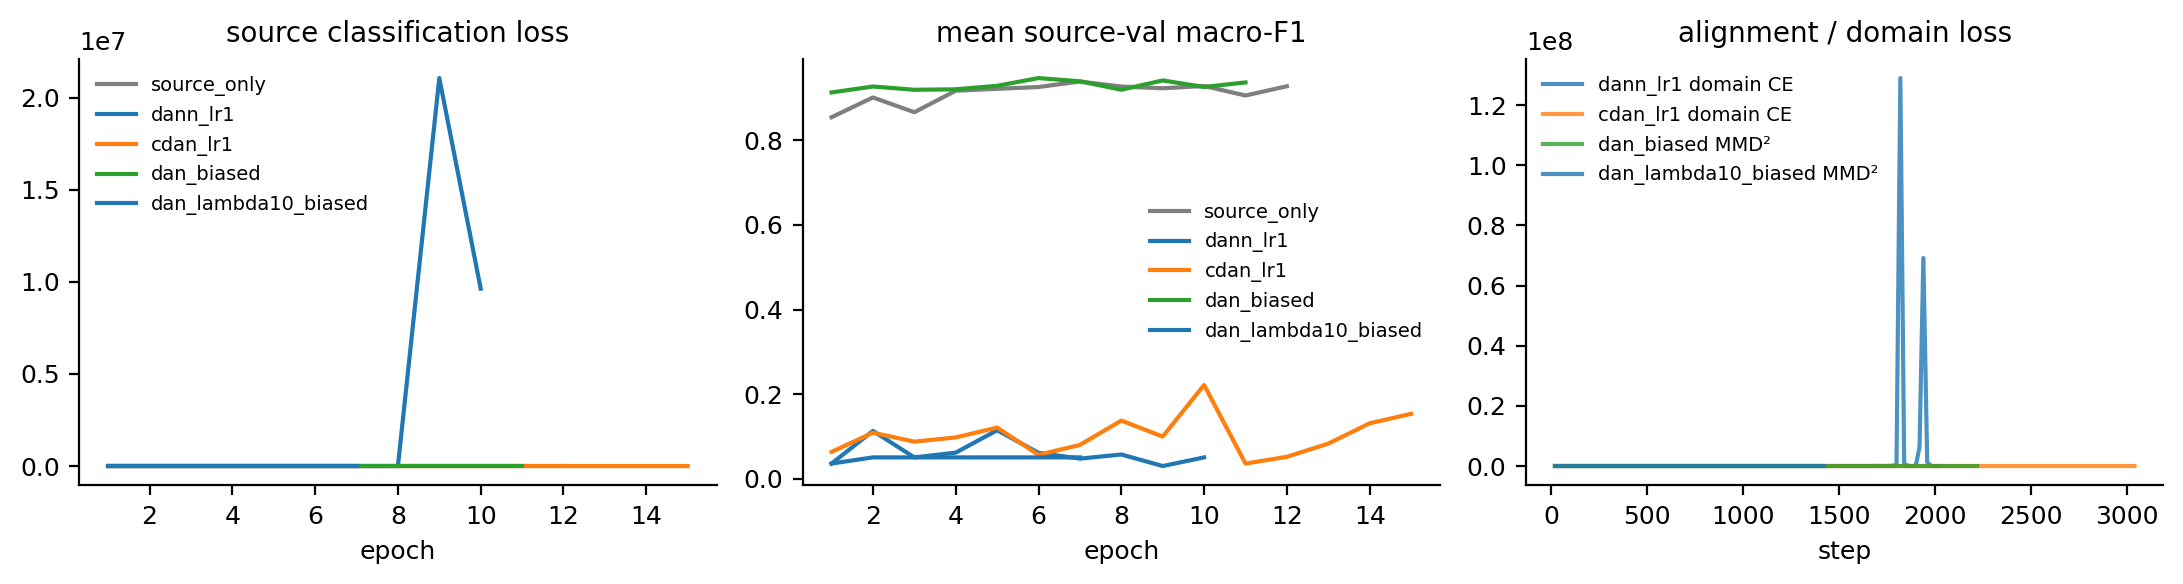
\includegraphics[width=0.99\textwidth]{task2__final_unstable_variants__training_curves.png}
\caption{Spec-exact DANN/CDAN and biased-MMD DAN: exploding domain and classification losses.}
\end{figure}

\begin{figure}[h]
\centering
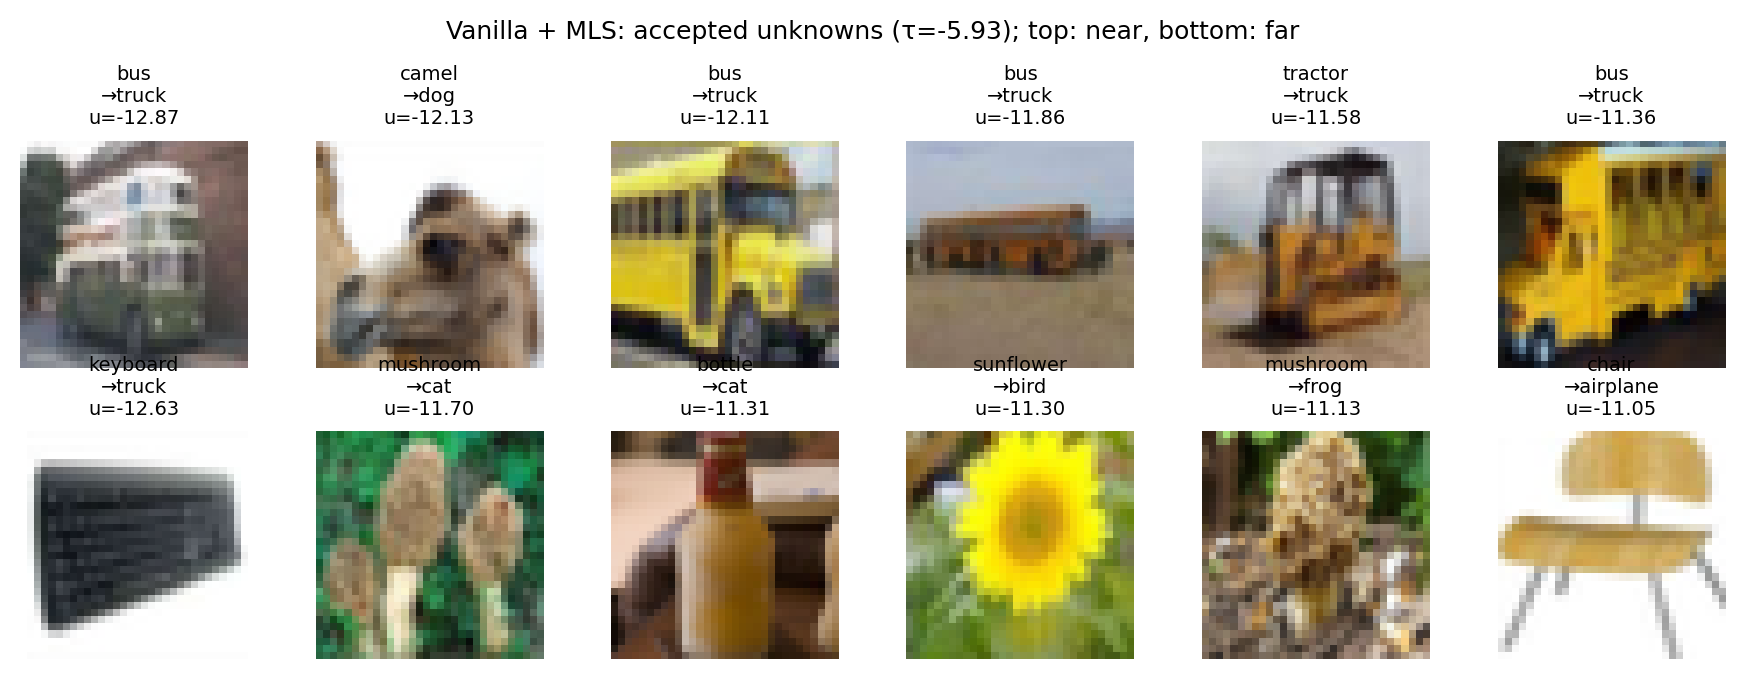
\includegraphics[width=0.85\textwidth]{task4__final__vanilla_mls_failures.png}
\caption{Most confidently accepted unknowns under Vanilla+MLS ($\tau=-5.93$); top row near, bottom row far, with unknown
class, predicted CIFAR-10 class and score.}
\end{figure}

\begin{table}[h]
\centering\small
\caption{Task 1 cue-conflict decisions per class pair and direction (shape/texture/other) for ResNet-50 (R), ViT-B/16 (V)
and the CLIP head (C); each cell lists $N_{\rm shape}/N_{\rm texture}/N_{\rm other}$.}
\label{tab:pairs}
\setlength{\tabcolsep}{4pt}
\input{pairs_table}
\end{table}

\begin{figure}[h]
\centering
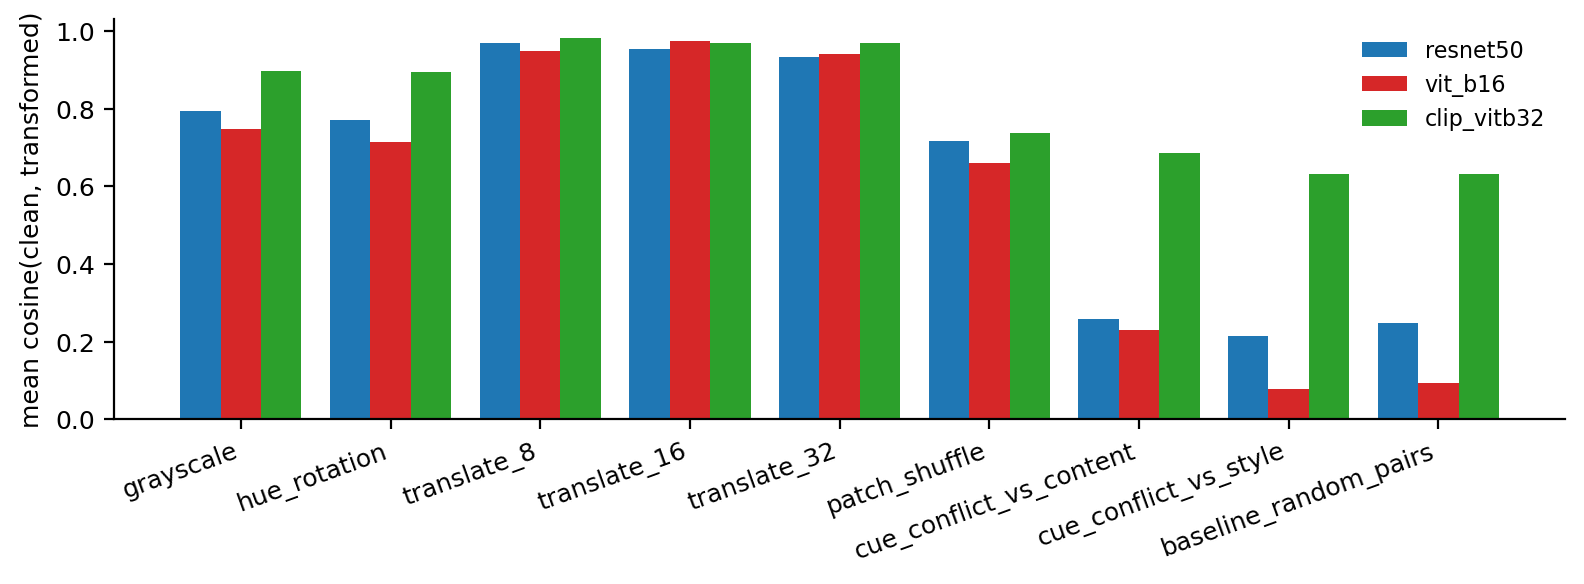
\includegraphics[width=0.75\textwidth]{task1__figures__representation_stability.png}
\caption{Task 1 representation stability per intervention and backbone.}
\end{figure}

\paragraph{Reproducibility.} Every table maps to a file: Task 1 \path{task1/results/*.csv}; Task 2
\path{task2/results/final_main}, \path{final_lambda_study}, \path{final_unstable_variants}; Task 3
\path{task3/results/final_main}, \path{final_rho_study}, \path{source_diagnostics}; Task 4 \path{task4/results/final}.
Commands are listed in the repository README.
\end{document}
